\def\lecture{2}
\clearpage \noindent\begin{tabularx}{\linewidth}{|X|}
\hline \vskip -2mm
{\sf 信号与系统} \hfill August 29, 2011 \\
{\centering \sf \large Lecture \lecture:
信号与系统\footnote{根据课件修正} \\ }
\textit{Lecturer: 王磊 \hfill Scriber: 戴唯思}\\ \hline
\end{tabularx}
\setcounter{section}{0}
\renewcommand{\thepage}{\lecture -\arabic{page}}


\section{一维信号的表示}

    \begin{description}
        \item[连续信号] 用$t$表示连续的时间自变量: $x(t)$
        \item[离散信号] 用$n$表示时间自变量: $x(n)$ or $x[n]$
    \end{description}

\section{信号的能量与功率}

    \subsection{连续时间信号的能量和功率}

    连续时间信号$x(t)$在$t_1\leq t\leq t_2$区间的\textbf{能量}定义为
    \[ E=\int_{t_1}^{t_2}|{x(t)}|^2\d t \]
    \textbf{平均功率}定义为
    \[ P=\frac{1}{t_2-t_1}\int_{t_1}^{t_2}|x(t)|^2\d t \]
    其中, $x(t)$为复函数.

    \subsection{离散时间信号的能量和功率}

    离散时间信号在$n_1\leq n\leq n_2$区间的\textbf{能量}定义为
    \[ E=\sum_{n=n_1}^{n_2}|x[n]|^2 \]
    \textbf{平均功率}为
    \[ P=\frac{1}{n_2-n_1+1}\sum_{n=n_1}^{n_2}|x[n]|^2 \]

    \subsection{无限区间上信号的能量和功率}

    \begin{table}[h]\centering
        \caption{无限区间上信号的能量和功率}
        \label{tab:2:universal-energy-and-power}
        \begin{tabular}{ccc} \toprule
            & 连续时间信号 & 离散时间信号 \\ \midrule
            总能量 & $ E_\infty=\lim_{T\to \infty}\int_{-T}^T|x(t)|^2\d t=\int_{-\infty}^\infty|x(t)|^2\d t $ & $E_\infty=\lim_{N\to \infty}\sum_{-N}^N|x[n]|^2=\sum_{-\infty}^\infty|x[n]|^2$\\ 
            平均功率 & $P_\infty=\lim_{T\to \infty}\frac{1}{2T}\int_{-T}^T|x(t)|^2\d t$ & $P_\infty=\lim_{N\to \infty}\frac{1}{2N+1}\sum_{-N}^N|x[n]|^2$ \\ \bottomrule
        \end{tabular}
    \end{table}

    \subsection{三类重要信号}
    
    \begin{itemize}
        \item \textbf{能量信号} 总能量有限: $E_\infty<\infty, P_\infty=0$
        \item \textbf{功率信号} 总能量无限, 平均能量有限: $E_\infty=\infty, 0<P_\infty<\infty$
        \item 总能量和平均功率都是无限的: $E_\infty=\infty, P_\infty=\infty$ \\
            这个世界上不存在
    \end{itemize}

\section{信号的自变量变换}

    \subsection{时移变换(time shift)}

        \[x(t)\to x(t-t_0)\]

        信号向右平移$t_0$.

    \subsection{反转变换}

        \[x(t)\to x(-t)\]

        信号以$t=0$为轴反转.

    \subsection{尺度变换}

        \[x(t)\to x(at)\]

        $a>1$时, $x(at)$是将$x(t)$在时间上压缩. $0<a<1$时, $x(at)$是将$x(t)$在时间上扩展.

        \subsubsection{离散信号的抽取}

            离散信号的尺度变换表现为对离散信号的抽取.

            \begin{figure}[h]\centering
                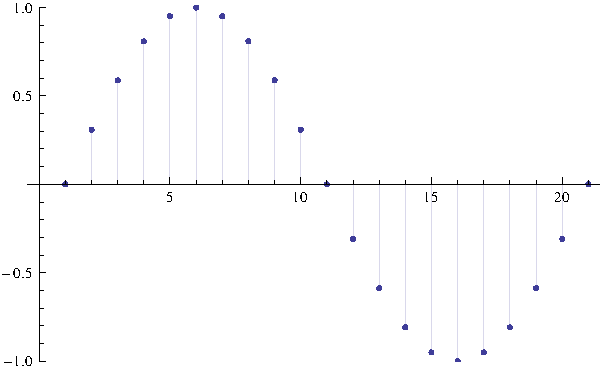
\includegraphics[width=6cm]{signals_chaps/lect2_inc/dt-time-shift-o.pdf} \raisebox{1.8cm}{$\to$} 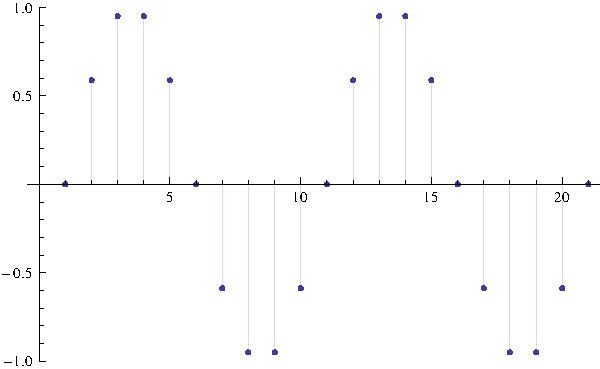
\includegraphics[width=6cm]{signals_chaps/lect2_inc/dt-time-shift-a.pdf}
                \caption{$\sin[0.1n\pi]$和$\sin[0.2n\pi]$}
                \label{fig:2:dt-time-shift-example}
            \end{figure}

    \subsection{综合}

        $x(t)\to x(\alpha t+\beta)$的一般过程:
        \begin{enumerate}
            \item 首先根据$\beta$的值将$x(t)$延时或超前(平移);
            \item 根据$\alpha$的值对延时或超前的信号做尺度变换;
            \item 如果$\alpha<0$则做时间反转;
            \item 用特殊点(零点, 端点和节点)验证.
        \end{enumerate}

\section{信号的周期性和奇偶性}

    \subsection{周期信号}

        \textbf{周期信号}满足对于全部的$t$或$n$, 存在$T\neq 0$或者$N\neq 0$使得$x(t)=x(t+T)$或者$x[n]=x[n+N]$成立, 其中$T$或$N$称为信号的\textbf{周期}.

        $2T, 3T, 4T,\cdots$或$2N, 3N, 4N, \cdots$也是信号的周期. 满足此关系的正实数(正整数)中最小的一个称为信号的\textbf{基波周期}, 表示为$T_0$或$N_0$.

        $x(t)=C$可以视为周期信号, 但基波周期没有明确的定义. $x[n]$的基波周期$N_0=1$.

    \subsection{信号的奇偶性}

        满足$x(-t)=x(t)$的信号是\textbf{偶信号}; 满足$x(-t)=-x(t)$的信号是\textbf{奇信号}.

        \subsubsection{一个神奇的规律}

            任何信号都能分解成一个偶信号与一个奇信号之和:

            \[x(t)=x_e(t)+x_o(t)\]
            \[x_e(t)=\frac{1}{2}[x(t)+x(-t)]\]
            \[x_o(t)=\frac{1}{2}[x(t)-x(-t)]\]

\section{几种基本信号}

    \subsection{正弦信号(Sine Wave, or sinusoid)}

        一般的正弦信号:

        \[x(t)=A\cos(\omega_0t+\phi)=\frac{A}{2}\e^{j\phi}\e^{j\omega_0t}+\frac{A}{2}\e^{-j\phi}\e^{-j\omega_0t} \]



\iffalse

\section{图片来源}

    图片来自Baraniuk, Richard. "Signals and Systems." Connexions. August  2, 2010. \url{http://cnx.org/content/col10064/1.12/}.

\fi
